\chapter{Simulations and Results}

The five algorithms where tested on different kind of maps and compared on three major performance indexes. Since our goal is to perform the coverage in the shortest time possible, minimize the total energy spent and also don't have redundant robots that do not produce a significant contribution to the coverage, the comparison criteria are based on:
\begin{itemize}
\item  Longest path (among all the robots) - $\max(\ell_i)$
\item  Total length of paths (sum over all the robots) -  $\sum(\ell_i)$
\item  Standard deviation of the paths lengths - $\sigma(\ell_i)$
\end{itemize}

The experimental phase is divided in two sections. In the first phase we analyse the algorithms behaviour in maps with random obstacles and compare the performances. The aim is to check among the different algorithms which one performs better in each situation. In the second phase instead the aim is to identify the optimal number of robots for a given map size so all the algorithm are tested varying the number of robots. The maps considered in this second phase are obstacle-free.
For a navigation graph $G_N(E,V)$ the standard coverage is said to be completed when all the vertices have been visited at least once, in formulas:

\begin{equation}
\min_i c(v_i) \geqslant 1 \qquad \forall v_i \in V
\end{equation}

Since some online algorithms due to their nature exhibit a more efficient behaviour on multiple coverages, i.e. patrolling, these algorithms have been tested also for $\min c \geqslant C$ where $C$ is greater than one.

For the first phase on grid maps with random obstacles, let's differentiate the three types of maps used in the algorithm by defining an obstacle index $\upomega$. The reference figures are Fig. \ref{fig:obstGrid1}, Fig. \ref{fig:obstGrid2} and Fig.\ref{fig:obstGrid3}.

\begin{figure}[H] 
  \label{fig:grid_types2} 
  \begin{minipage}[b]{0.32\linewidth}
    \centering
    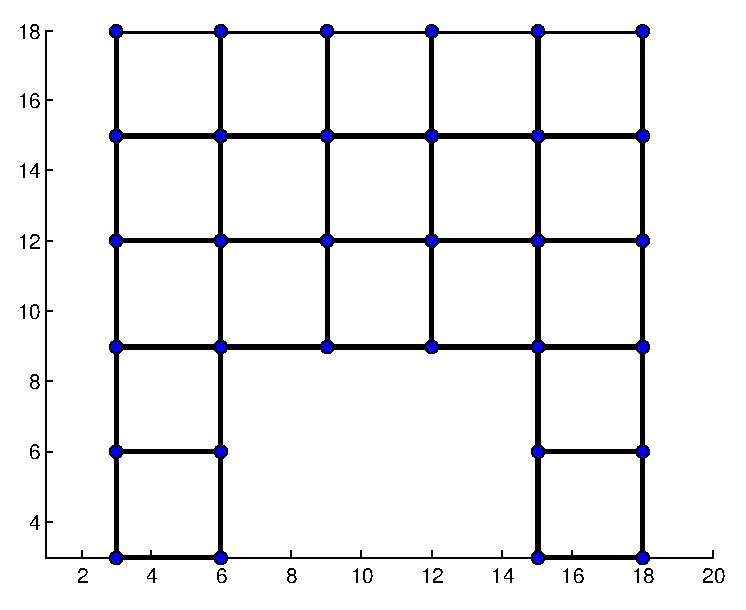
\includegraphics[width=0.8\textwidth]{6x6_Sparse1_1}
    \caption{$\upomega$=1}
    \label{fig:obstGrid1}
    \vspace{1ex}
  \end{minipage}
  \begin{minipage}[b]{0.32\linewidth}
    \centering
    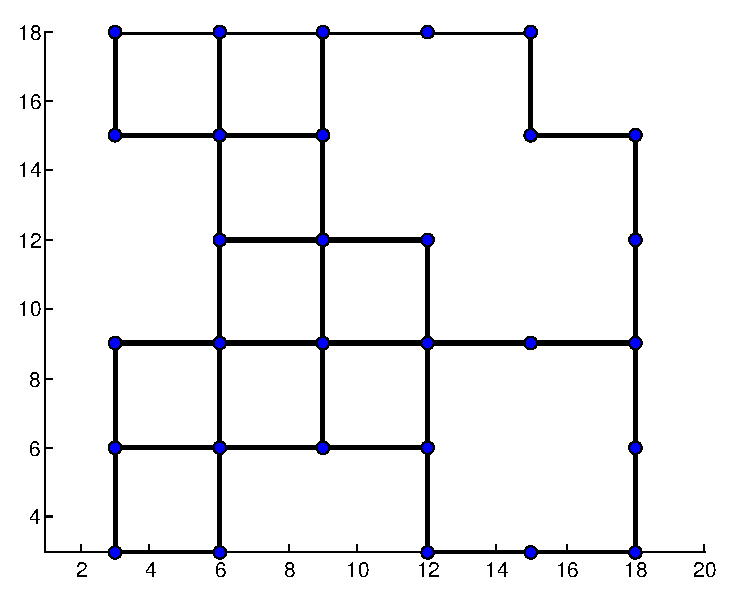
\includegraphics[width=0.8\textwidth]{6x6_Sparse2_1}
    \caption{$\upomega$=2}
    \label{fig:obstGrid2}
    \vspace{1ex}%%
  \end{minipage}
    \begin{minipage}[b]{0.32\linewidth}
    \centering
    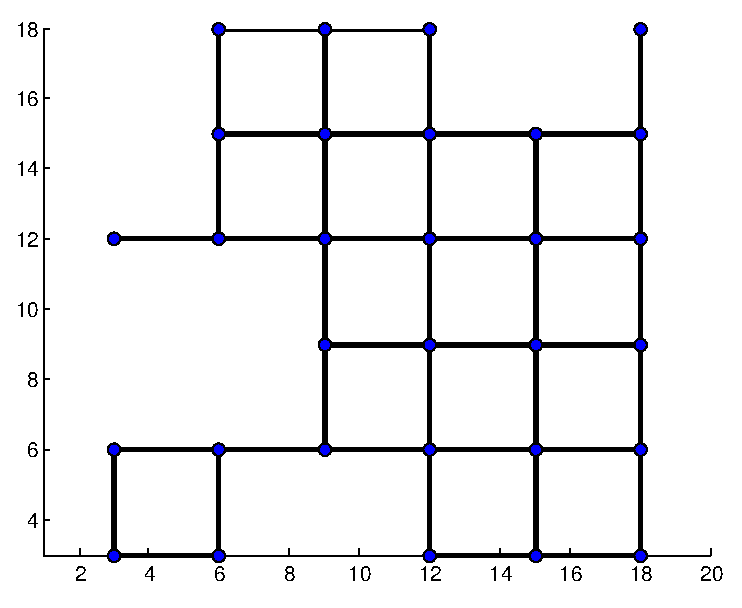
\includegraphics[width=0.8\textwidth]{6x6_Sparse3_2}
    \caption{$\upomega$=3}
    \label{fig:obstGrid3}
    \vspace{1ex}%%
  \end{minipage}
\end{figure}

Basically for $\upomega=0$ we have an obstacle-free map. For  $\upomega=1$ we have a map without internal holes and $\delta (G)=2$. For $\upomega=2$ we have a map with internal holes and still $\delta (G)=2$. For  $\upomega=3$ we have a map with internal holes and $\delta (G)=1$.
Tp test the algorithms the following simulation were performed:
\begin{description}
\item[\textbf{Set 1.}] Increasing map size: 4x4 Map, 6x6 Map, 8x8 Map
\item[\textbf{Set 2.}] Increasing $\upomega$:  $\upomega=1$, $\upomega=2$,  $\upomega=3$
\item[\textbf{Set 3.}] Increasing number of robots: 2 robots, 4 robots, 6 robots
\item[\textbf{Set 4.}] Increasing number of min-count per vertex: \mbox{$\min c=1$}, \mbox{$\min c =2$}, \mbox{$\min c =5$}, \mbox{$\min c =10$}
\end{description}

For each grid five different samples where tested and the result reported in the tables is the mean of the five simulations.

In the second phase to identify the best number of robots, three grid-maps of increasing size were tested, in particular the grids are of size: 5x5, 10x10, 15x15. For all the grids ten different simulations were performed increasing the number of quadcopters used, from a single robot coverage to a multi-robot coverage with 10 agents. For all the experiments the cells considered have a side of 2 m. In the following figures are presented 2 examples of coverage.

\begin{figure}[h] 
  \label{fig:finalPaths} 
  \begin{minipage}[b]{0.55\linewidth}
    \centering
    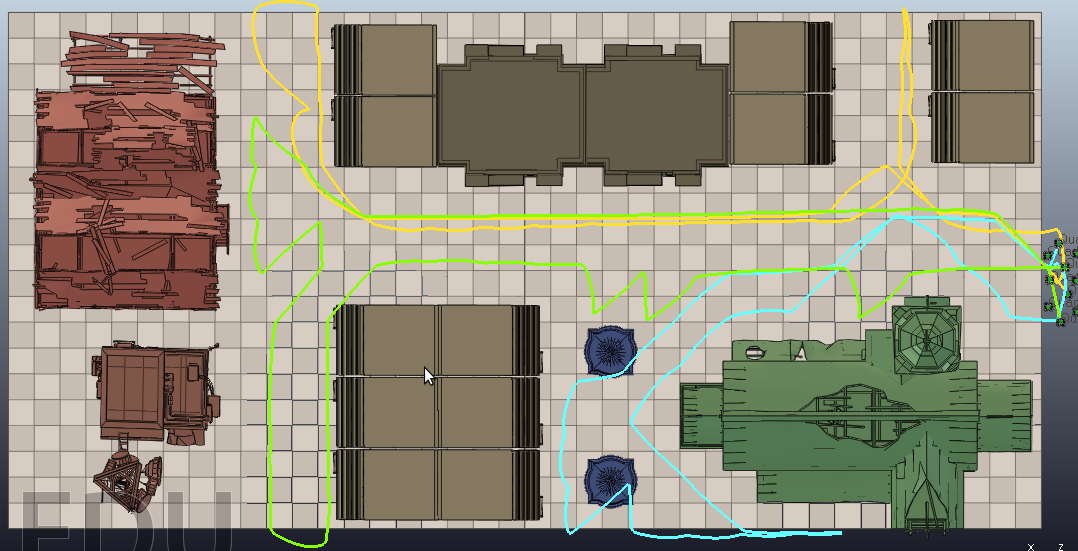
\includegraphics[width=\textwidth]{greedy_FW_newPlanningAlg_2}
    \caption{City map using VRP w/ F.W.}
    \label{fig:cityMap_VRP_sim}
    \vspace{1ex}
  \end{minipage}
  \begin{minipage}[b]{0.5\linewidth}
    \centering
    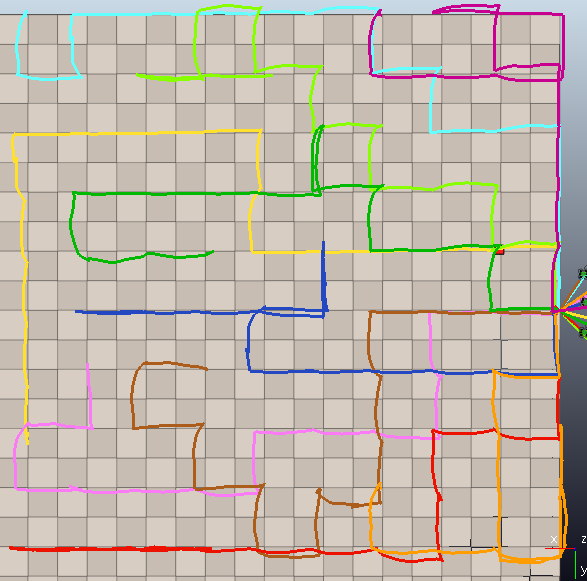
\includegraphics[width=0.65\textwidth]{NodeCount_10x10_10_2}
    \caption{Map 10x10 using N.C.}
    \label{fig:10x10_NC_sim}
    \vspace{1ex}%%
  \end{minipage}
%  \begin{minipage}[b]{0.5\linewidth}
%    \centering
%    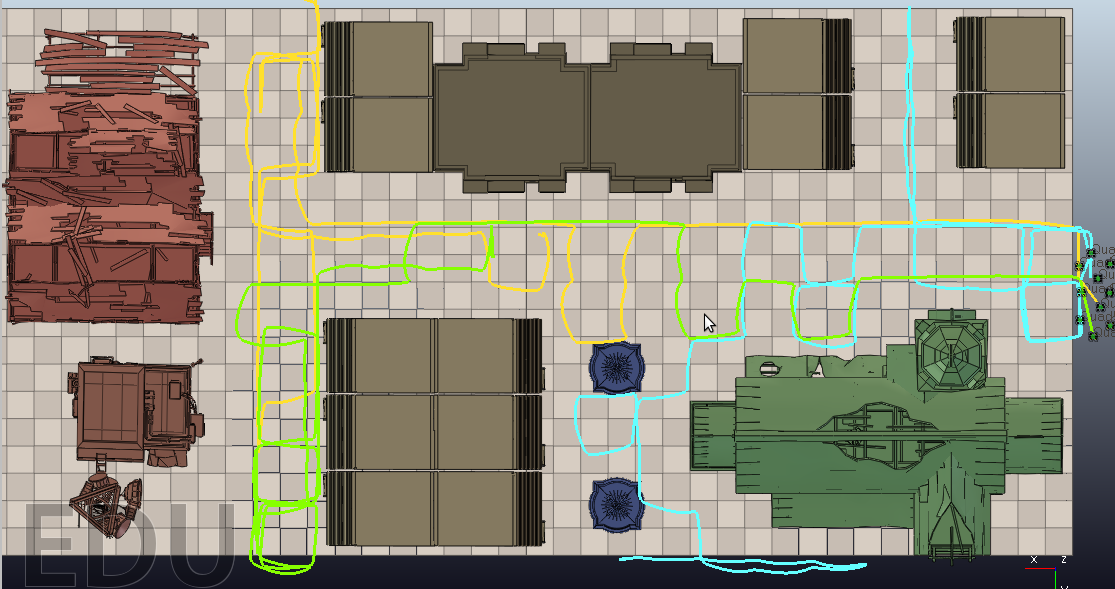
\includegraphics[width=\textwidth]{LRTAStar_new_planningAlg}
%    \caption{City map using LRTA*} 
%    %\label{fig:cellDec_pic3}
%    \vspace{4ex}
%  \end{minipage}
%  \begin{minipage}[b]{0.5\linewidth}
%    \centering
%    %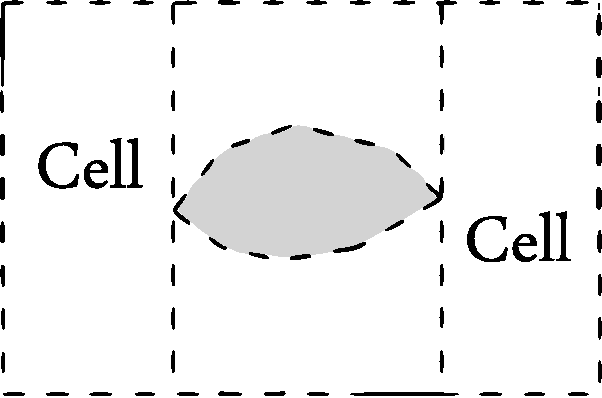
\includegraphics[width=0.7\textwidth]{boustrophedon_1}
%    \caption{4th path image}
%    %\label{fig:cellDec_pic4}
%    \vspace{4ex}%% 
%  \end{minipage} 
\end{figure}

\section{Algorithms Comparison}

\subsection{Single robot behaviour}
\label{sec:singleRob}
Before jumping to the multi-robot case let's make some considerations on the single-robot coverage. The extension of a single-robot coverage algorithm to the multi-robot case is not straightforward and at a first glance some of the results in the next sections may appear counterintuitive. For example as stated before LRTA* suffers a performance degradation in the multi-robot case. So, even if the scope of this thesis is focused on multi-robot coverage, to prove that the algorithms developed are fully functional and have a behaviour congruent with the result found in literature, simulations were performed also for a single-robot configuration using a 4x4 grid map. 


Since an interesting trend can be observed when changing the number of minimum visits per vertex we tested the algorithms for 4 different values of $\min c$.  The results are presented in table \ref{tab:singleRobResults}.

% Please add the following required packages to your document preamble:
% \usepackage{booktabs}
% \usepackage{multirow}
\begin{table}[H]
\centering
\begin{tabular}{@{}ccc@{}}
\toprule
Algorithm                                    & $\min c$  & $\ell(P)$           \\ \midrule
\multirow{4}{*}{Node Count} &   10        &   178             \\
                                         &   5          &     98             \\
                                         &  2           &    51              \\
                                         &  1           &    17              \\ \midrule
\multirow{4}{*}{LRTA*}     &  10          &   160             \\
                                        &   5           &   79                \\
                                        &   2           &   35                \\
                                        &   1           &   17                 \\ \bottomrule
\end{tabular}
\qquad \qquad%adds some space between tables
\begin{tabular}{@{}ccc@{}}
\toprule
Algorithm                               & $\min c$  & $\ell(P)$           \\ \midrule
\multirow{4}{*}{Edge Count} &   10      &   250              \\
                                         &   5          &     134            \\
                                         &   2          &    75               \\
                                         &   1          &   34                \\ \midrule
\multirow{4}{*}{PatrolGRAPH*}&   10   &    178            \\
                                        &   5          &   108               \\
                                        &   2          &   57                 \\
                                        &   1          &   47                 \\ \bottomrule
\end{tabular}
\caption{Single-robot comparison for a 4x4 map and $\upomega=0$}
\label{tab:singleRobResults}
\end{table}



As we can see the LRTA* always perform equal or better than Node Counting. It is interesting to notice how approaching the single coverage, the difference between NC and LRTA* becomes less considerable, becoming eventually equally for \mbox{$\min c=1$}.
Comparing Edge Count and PatrolGRAPH* we can see how for \mbox{$\min c>1$} the latter always completes the patrolling in fewer steps, while for the single coverage instead Edge Counting turns out to be more efficient. This happens since, as can be observed in appendix \ref{app:firstSteps}, in the first steps of the algorithm PG* tends to make the robot go back to already visited vertices. The reason behind this behaviour relies in the fact that having computed a Probability Transition Matrix that ensures every vertex to be visited with a probability $p=\sfrac{1}{N}$, PG* in the initial transient phase spends more time visiting vertices with a low number of edges to make coincide the desired visit frequency with the actual one.
Apart from this we can notice how the paths length for NC and LRTA* are always smaller than the ones resulting from EC and PG*, and this is also true for the multi-robot case as we will see in the next sections, making clear that vertex-count oriented algorithms are more suitable for coverage purposes.

%%%%%%%%%%%%%%%%%%

\subsection{Node Counting}

In table \ref{tab:NC_results} are presented the results for the Node Counting algorithm.

% Please add the following required packages to your document preamble:
% \usepackage{booktabs}
% \usepackage{multirow}

\begin{table}[H]
%\setlength{\tabcolsep}{1.5em}
\centering
\begin{tabular}{@{}cccccccc@{}}
\toprule
Set                & \multicolumn{4}{c}{Parameters}  & \multicolumn{3}{c}{Results}              \\ \cmidrule(lr){2-5} \cmidrule(lr){6-8}
                   & $\upomega$ & \#Rob & Grid Size & $\min c$ & $\max(\ell_i)$ & $\sum(\ell_i)$ & $\sigma(\ell_i)$ \\ \midrule
\multirow{3}{*}{1} & 1           & 3     & 4x4       &   1     &   7        &  19       &   0.394   \\
                             & 1           & 3     & 6x6       &   1     &   20      &  60       &   0.673    \\
                             & 1           & 3     & 8x8       &   1     &   37      &  109     &   0.785    \\ \midrule
\multirow{3}{*}{2} & 1           & 3     & 6x6       &   1     &   20      &  58       &  0.605     \\
                             & 2           & 3     & 6x6       &   1     &   16      &  45       &  0.625     \\
                             & 3           & 3     & 6x6       &   1     &   19      &  55       &  0.394     \\ \midrule
\multirow{3}{*}{3} & 1           & 2     & 6x6       &   1     &   27      &  54       & 0.341       \\
                             & 1           & 4     & 6x6       &   1     &   14      &  54       & 0.615       \\
                             & 1           & 6     & 6x6       &   1     &   11      &  60       & 0.770       \\ \midrule
\multirow{4}{*}{4} & 1           & 3     & 6x6       &   10     &  114	&  338       & 1.414           \\
                             & 1           & 3     & 6x6       &   5     &  68      &   202   &   0.577        \\
                             & 1           & 3     & 6x6       &   2     &  30      &  89      &   0.816       \\
                             & 1           & 3     & 6x6       &   1    &  15     &   44     &   0.816       \\ \bottomrule
\end{tabular}
\caption{Results of the simulation for the Node Counting Alg.}
\label{tab:NC_results}
\end{table}



Despite it is the simplest of the algorithms considered it is surprisingly good for multi-robot coverage. For the simulation in Set 1 of increasing map size with $\upomega=1$ the LRTA* is the only other algorithm with similar performances, although in the 8x8 grid NC still performs better. Also for Sets 2 and 3 the two algorithms get similar results, but for the 6 robots case (Set 3), the Node Counting completes the coverage in fewer steps. 

%%%%%%%%%%%%%%%%%%

\subsection{Learning Real-Time A*}

In table \ref{tab:LRTA_results} are presented the results for the Learning Real-Time A* algorithm. As stated in section \ref{sec:LRTAstar} the update-rule of LRTA* is not triggered till the robot reaches the target vertex and this entails that multiple robots can make the same choice consequently not contributing in spreading the robots across the map. This disadvantage clearly emerges from the simulations where in almost all the cases the Node Counting achieves better results. This becomes even more noticeable in Set 4 for big values of $\min c$ where even if the difference between $\max (\ell_i)$ is not that big, thinking in terms of total energy spent by the swarm, $\sum(\ell_i)$, in LRTA* is significantly bigger (NC 338 vs. LRTA* 456).

% Please add the following required packages to your document preamble:
% \usepackage{booktabs}
% \usepackage{multirow}
\begin{table}[H]
\centering
\begin{tabular}{@{}cccccccc@{}}
\toprule
Set                & \multicolumn{4}{c}{Parameters}  & \multicolumn{3}{c}{Results}              \\ \cmidrule(lr){2-5} \cmidrule(lr){6-8}
                   & $\upomega$ & \#Rob & Grid Size & $\min c$ & $\max(\ell_i)$ & $\sum(\ell_i)$ & $\sigma(\ell_i)$ \\ \midrule
\multirow{3}{*}{1} & 1           & 3     & 4x4       &   1     &  7        &  24        &   0.558   \\
                             & 1           & 3     & 6x6       &   1     &   19      &  56       &   0.773    \\
                             & 1           & 3     & 8x8       &   1     &   43      &  125     &   0.558    \\ \midrule
\multirow{3}{*}{2} & 1           & 3     & 6x6       &   1     &   23      &  68       &  0.762     \\
                             & 2           & 3     & 6x6       &   1     &   20      &  60       &  0.490     \\
                             & 3           & 3     & 6x6       &   1     &   16      &  46       &  0.840     \\ \midrule
\multirow{3}{*}{3} & 1           & 2     & 6x6       &   1     &   26      &  50        & 0.624       \\
                             & 1           & 4     & 6x6       &   1     &   19      &  72       &  0.387      \\
                             & 1           & 6     & 6x6       &   1     &   15     &   85      &   0.725     \\ \midrule
\multirow{4}{*}{4} & 1           & 3     & 6x6       &   10   &  154    &  456      &   1.633         \\
                             & 1           & 3     & 6x6       &   5     &   96     &  286      &   1.00       \\
                             & 1           & 3     & 6x6       &   2     &   31     &   91      &  0.577        \\
                             & 1           & 3     & 6x6       &   1    &    18      &  53      &  0.816  \\ \bottomrule
\end{tabular}
\caption{Results of the simulation for the LRTA* Alg.}
\label{tab:LRTA_results}
\end{table}




%%%%%%%%%%%%%%%%%%

\subsection{Edge Counting}

The first thing we notice from the results in table \ref{tab:EC_results} is that average number of visits, and consequently also total length, of the Edge Counting algorithm is generally higher for any of the 4 test cases with respect to the previous to algorithms. The results are more in line with PatrolGRAPH* algorithms ones, also for what regards the $\sigma(\ell_i)$ that in Set 4 reaches values up to $\sigma=4.08$, while for the same set the maximum for LRTA* is $\sigma=1.6$. In general it comes out that for a single-coverage task (Sets 1-2-3) on average the Edge Counting is faster than PG*.  It is worth reminding anyway that in none of the previous coverage algorithm we have control over the frequency distribution of visits, so it is not possible for example to define an ``region priority'', which can instead be achieved using the PatrolGRAPH*.

% Please add the following required packages to your document preamble:
% \usepackage{booktabs}
% \usepackage{multirow}
\begin{table}[H]
\centering
\begin{tabular}{@{}cccccccc@{}}
\toprule
Set                & \multicolumn{4}{c}{Parameters}  & \multicolumn{3}{c}{Results}              \\ \cmidrule(lr){2-5} \cmidrule(lr){6-8}
                   & $\upomega$ & \#Rob & Grid Size & $\min c$ & $\max(\ell_i)$ & $\sum(\ell_i)$ & $\sigma(\ell_i)$ \\ \midrule
\multirow{3}{*}{1} & 1           & 3     & 4x4       &   1     &  18        &  52        &   0.605   \\
                             & 1           & 3     & 6x6       &   1     &   69      &  203       &   1.15    \\
                             & 1           & 3     & 8x8       &   1     &   142      &  422     &   1.32   \\ \midrule
\multirow{3}{*}{2} & 1           & 3     & 6x6       &   1     &   59      &  175       &  1.04     \\
                             & 2           & 3     & 6x6       &   1     &   56      &  167       &  0.860     \\
                             & 3           & 3     & 6x6       &   1     &   46      &  133       &  0.958     \\ \midrule
\multirow{3}{*}{3} & 1           & 2     & 6x6       &   1     &   75      &  148       &  0.974        \\
                             & 1           & 4     & 6x6       &   1     &  44      &   171     &    0.800           \\
                             & 1           & 6     & 6x6       &   1     &  42       &   244    &   1.06       \\ \midrule
\multirow{4}{*}{4} & 1           & 3     & 6x6       &   10   &  205     &  605     &    4.08   \\
                             & 1           & 3     & 6x6       &   5     &  145     &  430     &  2.38     \\
                             & 1           & 3     & 6x6       &   2     &  75      & 222      &  0.816        \\
                             & 1           & 3     & 6x6       &   1    &   63      & 188      &  0.816        \\ \bottomrule
\end{tabular}
\caption{Results of the simulation for the Edge Counting Alg.}
\label{tab:EC_results}
\end{table}



% Please add the following required packages to your document preamble:
% \usepackage{booktabs}
% \usepackage{multirow}
\begin{table}[H]
\centering
\begin{tabular}{@{}cccccccc@{}}
\toprule
Set                & \multicolumn{4}{c}{Parameters}  & \multicolumn{3}{c}{Results}              \\ \cmidrule(lr){2-5} \cmidrule(lr){6-8}
                   & $\upomega$ & \#Rob & Grid Size & $\min c$ & $\max(\ell_i)$ & $\sum(\ell_i)$ & $\sigma(\ell_i)$ \\ \midrule
\multirow{3}{*}{1} & 1           & 3     & 4x4       &   1     &  25       &  74       &   0.662   \\
                             & 1           & 3     & 6x6       &   1     &   65      &  192      &   0.908    \\
                             & 1           & 3     & 8x8       &   1     &   150     &  447     &   1.17    \\ \midrule
\multirow{3}{*}{2} & 1           & 3     & 6x6       &   1     &   61      &  182      &  0.836     \\
                             & 2           & 3     & 6x6       &   1     &   66      &  193      &  1.19     \\
                             & 3           & 3     & 6x6       &   1     &   69      &  204      &  1.39     \\ \midrule
\multirow{3}{*}{3} & 1           & 2     & 6x6       &   1     &  88       &  174      &  0.832        \\
                             & 1           & 4     & 6x6       &   1     &  51       &  201      &  0.852        \\
                             & 1           & 6     & 6x6       &   1     &  41       & 241       &  0.539           \\ \midrule
\multirow{4}{*}{4} & 1           & 3     & 6x6       &   1     &  180     &   533     &    3.366        \\
                             & 1           & 3     & 6x6       &   2     &  114     &  339      &   0.816        \\
                             & 1           & 3     & 6x6       &   5     &  70      &   207      &   0.816       \\
                             & 1           & 3     & 6x6       &   10   &  66      &    198     &  0        \\ \bottomrule
\end{tabular}
\caption{Results of the simulation for the PatrolGRAPH* Alg.}
\label{tab:PG_results}
\end{table}



%%%%%%%%%%%%%%%%%%

\subsection{PatrolGRAPH*}

Observing the PatrolGRAPH* results in table \ref{tab:PG_results} we find that the values for Set 3 are against the trend of all the previous algorithms. While previously for growing $\upomega$ the $\max(\ell_i)$ index is decreasing, in the PG* case smaller $\delta(G)$ cause longer coverage paths. This behaviour can be explained with the same reasoning done for the single-robot case in section \ref{sec:singleRob} recalling that the PG* algorithm will spend more time on vertices with small number of edges to ensure that on a short term time horizon the expected and actual frequency distribution concide. It is worth noting that on the long run the PG*, ensuring a uniform frequency distribution, performs better than Edge Counting as we can see the case of $\min c=10$ of Set 4.


%%%%%%%%%%%%%%%%%%

\subsection{VRP Greedy with Floyd-Warshall}

For the reasons explained in the previous chapter regarding computation time and quality of the solutions, the VRP Greedy with Floyd-Warshall is the only offline algorithm that will be used in the simulations. The results are presented in table \ref{tab:VRP_FW_results1}. Since the result of the Greedy algorithm is deterministic there is no point in considering $\min c>1$, as the total path length can be easily evaluated by multiplying the result indexes of the single-coverage case by the number of coverages.

% Please add the following required packages to your document preamble:
% \usepackage{booktabs}
% \usepackage{multirow}
\begin{table}[H]
\centering
\begin{tabular}{@{}ccccccc@{}}
\toprule
Set                & \multicolumn{3}{c}{Parameters}  & \multicolumn{3}{c}{Results}              \\ \cmidrule(lr){2-4} \cmidrule(lr){5-7}
                   & $\upomega$ & \#Rob & Grid Size & $\max(\ell_i)$ & $\sum(\ell_i)$ & $\sigma(\ell_i)$ \\ \midrule
\multirow{3}{*}{1} & 1           & 3     & 4x4       &    10        &  25        &   1.72   \\
                             & 1           & 3     & 6x6       &      20      &  53       &   2.10    \\
                             & 1           & 3     & 8x8       &     33      &  90      &   2.52    \\ \midrule
\multirow{3}{*}{2} & 1           & 3     & 6x6       &      17      &  48       &  1.39     \\
                             & 2           & 3     & 6x6       &      19      &  51       &  2.32     \\
                             & 3           & 3     & 6x6       &     20      &  55       &  1.70     \\ \midrule
\multirow{3}{*}{3} & 1           & 2     & 6x6       &     24      &  45       &   1.80        \\
                             & 1           & 4     & 6x6       &     16       &  59       &   1.27            \\
                             & 1           & 6     & 6x6       &     15      &  67        &    4.18        \\ \bottomrule                             
\end{tabular}
\caption{Results of the simulation for the VRP w/ F.W. Alg.}
\label{tab:VRP_FW_results1}
\end{table}



Comparing the VRP results with the Node Counting ones, which has been found to be the simplest yet the best algorithm so far, we can observe how Node Counting is surprisingly powerful. There are few cases for which VRP is better than NC, and this occur occur mainly with big maps (8x8 grid) and low $\upomega$. We can observe the same results also for the simulation in the next section, and deduce then that the Greedy VRP performs better in obstacle-free maps, with a bigger ``manoeuvring space''.

\subsection{Comparison Conclusions}
From the analysis carried in this chapter it emerged how on average the best solution for the single-coverage multi-robot problem is produced by the Node Counting algorithm. First of all is interesting to notice that a (simple) offline method (no heuristic post-optimisation), does not necessarily produce a better solution than a (simple) online method. A very basic swarm rule (NC) can achieve better results than the a fairly complex routing algorithm and also, being an online method, NC is more flexible and suitable for autonomous distributed systems than VRP.
This result against the trend of the results found in literature for the single-robot coverage makes clear how the extension of current coverage approaches to the multi-robot case is not trivial and requires an accurate study on communication protocols between robots and collective behaviour in general.



\pagebreak



\section{Finding the optimal number of robots}
To find the optimal number of robots the map tested were: the city environment map and 3 increasing size obstacle-free square maps: 5x5, 10x10, 15x15. After normalising the result parameters, the method used for establishing the optimal number of robots is evaluating the output of a weighted loss function $\mathscr{L}$ where three $\lambda$ weight are assigned to each of the result parameters. In formulas, for a generic number of robots $R$:

\begin{equation}
\mathscr{L}_R(\lambda, \ell_i)=\lambda_1 \cdot \max(\ell_i)_N + \lambda_2 \cdot \sum(\ell_i)_N + \lambda_3 \cdot \sigma(\ell_i)_N
\end{equation}

Where subscript $N$ stands for normalised, and the best configuration will be the one that satisfies the following formula:

\begin{equation}
R_{best} = \arg\min_R \mathscr{L}_R(\lambda, \ell_i)
\end{equation}
 
By acting on the parameters we can set a  lexicographical order that meets the objective we want to achieve. The $\lambda$ parameters where obtained with a simple tuning based on the fact that the most important parameter is $\lambda_1$ since it weights $max(\ell_i)$ that defines the coverage completion time, and we want to minimize it. Then on a second level we want that the total energy spent by the swarm is minimized and at last we don't want a big disparity between paths lengths since it means that are some redundant robots. The parameters of the online and offline algorithms are not the same since in the online algorithms, till the coverage is completed, each robot performs the same number of steps, so $\lambda_3$ was set to a very small value with respect to the other two parameters.
By taking advantage of the analysing performed in the previous section the simulations for this case will be run only for the Node Counting and VRP algorithms.
In the following figures all the values in the graphs will be also represented as normalised. Due to the long execution times of the Node Counting (the deterministic solution of the Greedy is almost instant), the two algorithms will be compared for maps sizes not greater than 15x15.

%%%%%%%%%%%%%%%%%%%%

\subsection{Node Counting}
A common trend in all the plots is that the maximum path length $\max (\ell_i)$ always decreases with the increasing number of robots, which is an expected intuitive result. Nevertheless there is point where increasing the number of robots is no more convenient due to the consequent increase of the total paths length $\sum (\ell_i)$. An interesting result that can be observed in the profile of the total length curve is that there are some local minima that for larger sizes of the map occur in correspondence of a higher number of robots.

%\begin{figure}[H]
\centering
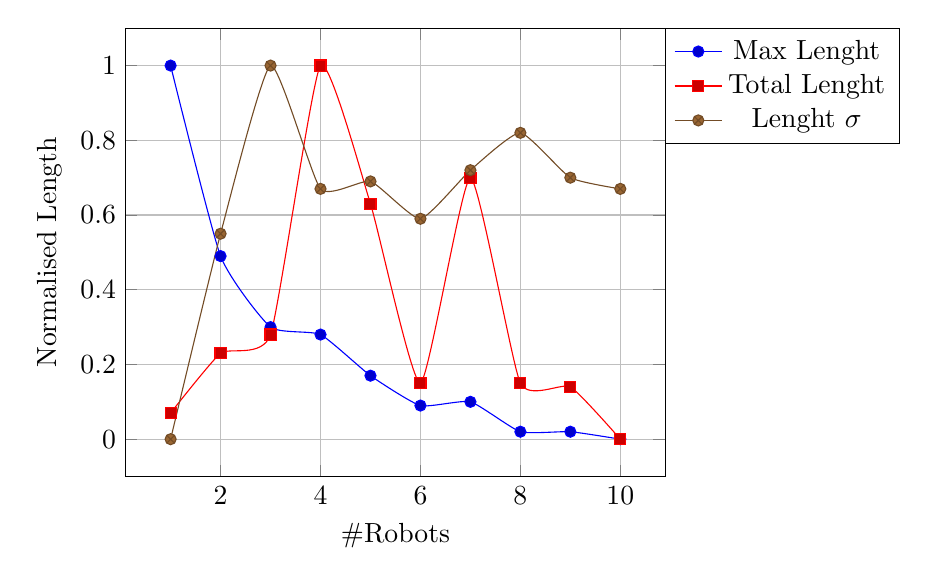
\begin{tikzpicture}
	\begin{axis}[
%		height=9cm,
%		width=9cm,
		grid=major,
                legend style = {at={(1,1)}, anchor=north west},
		xlabel=\#Robots,
		ylabel=Normalised Length,
		smooth,
		tension=0.3
	]

	\addplot coordinates {
(1, 1.00)
(2, 0.49)
(3, 0.30)
(4, 0.28)
(5, 0.17)
(6, 0.09)
(7, 0.10)
(8, 0.02)
(9, 0.02)
(10, 0.00)
	};
	\addlegendentry{Max Lenght}

	\addplot coordinates {
(1, 0.07)
(2, 0.23)
(3, 0.28)
(4, 1.00)
(5, 0.63)
(6, 0.15)
(7, 0.70)
(8, 0.15)
(9, 0.14)
(10, 0.00)
	};
	\addlegendentry{Total Lenght}

	\addplot coordinates {
(1, 0.00)
(2, 0.55)
(3, 1.00)
(4, 0.67)
(5, 0.69)
(6, 0.59)
(7, 0.72)
(8, 0.82)
(9, 0.70)
(10, 0.67)
	};
	\addlegendentry{Lenght $\sigma$}
	\end{axis}
\end{tikzpicture}
\caption{Variation of the performance indexes increasing the number of robots, for the 15x15 grid using the Node Counting algorithm}
\end{figure}


\begin{figure}[H]
\centering
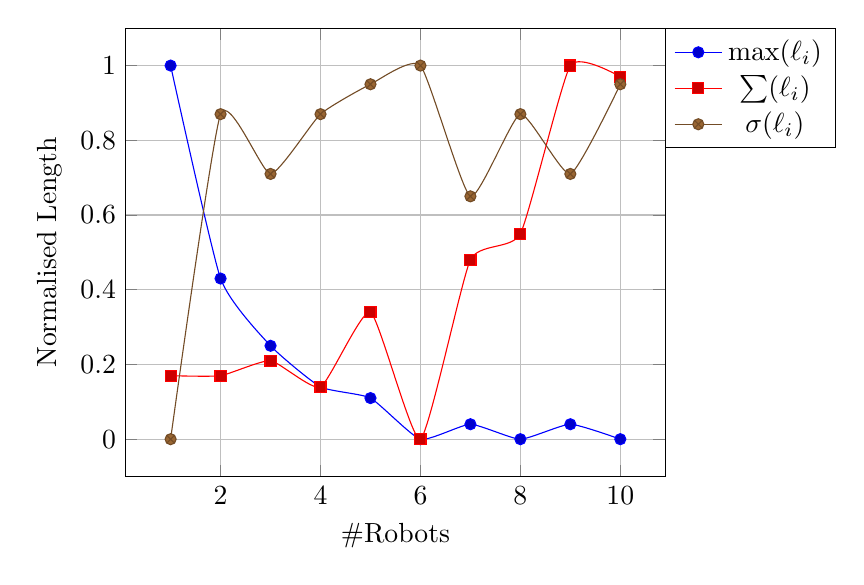
\begin{tikzpicture}
	\begin{axis}[
%		height=9cm,
%		width=9cm,
		grid=major,
                legend style = {at={(1,1)}, anchor=north west},
		xlabel=\#Robots,
		ylabel=Normalised Length,
		smooth,
		tension=0.3
	]

	\addplot coordinates {
(1, 1.00)
(2, 0.43)
(3, 0.25)
(4, 0.14)
(5, 0.11)
(6, 0.00)
(7, 0.04)
(8, 0.00)
(9, 0.04)
(10, 0.00)
	};
	\addlegendentry{$\max(\ell_i)$}

	\addplot coordinates {
(1, 0.17)
(2, 0.17)
(3, 0.21)
(4, 0.14)
(5, 0.34)
(6, 0.00)
(7, 0.48)
(8, 0.55)
(9, 1.00)
(10, 0.97)
	};
	\addlegendentry{$\sum(\ell_i)$}

	\addplot coordinates {
(1, 0.00)
(2, 0.87)
(3, 0.71)
(4, 0.87)
(5, 0.95)
(6, 1.00)
(7, 0.65)
(8, 0.87)
(9, 0.71)
(10, 0.95)
	};
	\addlegendentry{$\sigma(\ell_i)$}
	\end{axis}
\end{tikzpicture}
\caption[Perform. indexes increasing the \#robots, 5x5 grid using NC]{Performance indexes increasing the num. of robots, 5x5 grid using NC}
\end{figure}


\begin{figure}[H]
\centering
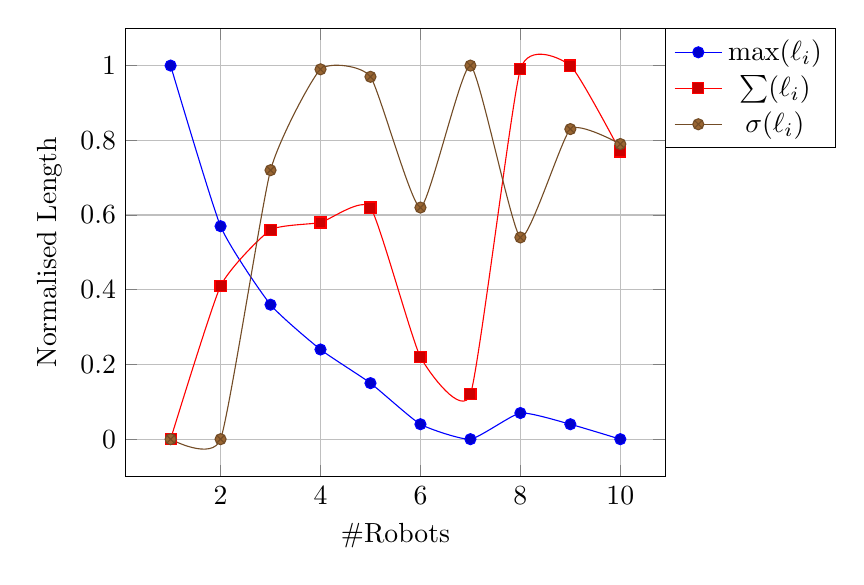
\begin{tikzpicture}
	\begin{axis}[
%		height=9cm,
%		width=9cm,
		grid=major,
                legend style = {at={(1,1)}, anchor=north west},
		xlabel=\#Robots,
		ylabel=Normalised Length,
		smooth,
		tension=0.3
	]

	\addplot coordinates {
(1, 1.00)
(2, 0.57)
(3, 0.36)
(4, 0.24)
(5, 0.15)
(6, 0.04)
(7, 0.00)
(8, 0.07)
(9, 0.04)
(10, 0.00)
	};
	\addlegendentry{$\max(\ell_i)$}

	\addplot coordinates {
(1, 0.00)
(2, 0.41)
(3, 0.56)
(4, 0.58)
(5, 0.62)
(6, 0.22)
(7, 0.12)
(8, 0.99)
(9, 1.00)
(10, 0.77)
	};
	\addlegendentry{$\sum(\ell_i)$}

	\addplot coordinates {
(1, 0.00)
(2, 0.00)
(3, 0.72)
(4, 0.99)
(5, 0.97)
(6, 0.62)
(7, 1.00)
(8, 0.54)
(9, 0.83)
(10, 0.79)
	};
	\addlegendentry{$\sigma(\ell_i)$}
	\end{axis}
\end{tikzpicture}
\caption[Perform. indexes increasing the \#robots, 10x10 grid using NC]{Performance indexes increasing the num. of robots, 10x10 grid using NC}
\end{figure}

So for the Node Counting algorithm we have that for a 5x5 map the best number of robots is 6, for the 10x10 map is 7 and for the 15x15 map is 10. The bigger leap between the last two results derives from the fact that a linear increase in the map side obviously produces a quadratic increase in the map area, thus on the size of the navigation graph. Even though no precise pattern is emerging from the relationship between number of robots and size of the map, this results give anyway an idea about the order of magnitude of the robots necessary for coverage for increasing map size.


\begin{figure}[H]
\centering
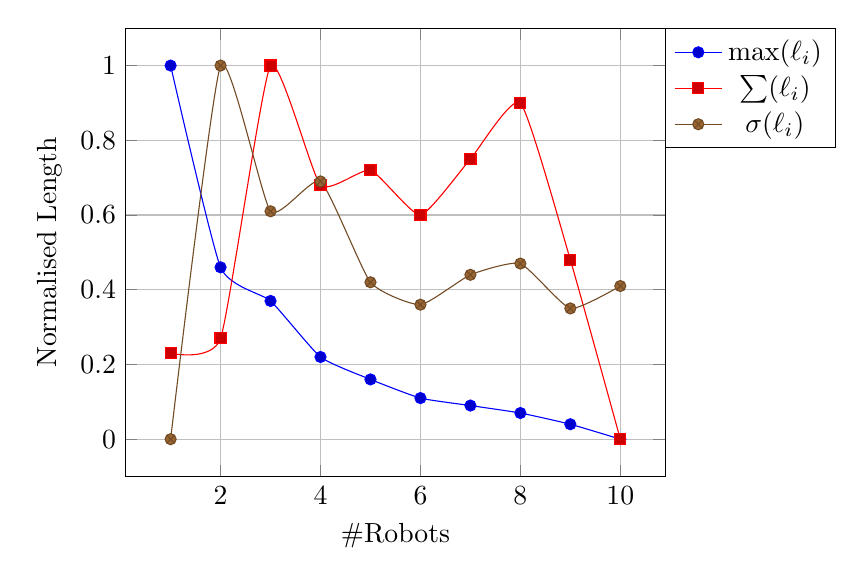
\begin{tikzpicture}
	\begin{axis}[
%		height=9cm,
%		width=9cm,
		grid=major,
                legend style = {at={(1,1)}, anchor=north west},
		xlabel=\#Robots,
		ylabel=Normalised Length,
		smooth,
		tension=0.3
	]

	\addplot coordinates {
(1, 1.00)
(2, 0.46)
(3, 0.37)
(4, 0.22)
(5, 0.16)
(6, 0.11)
(7, 0.09)
(8, 0.07)
(9, 0.04)
(10, 0.00)
	};
	\addlegendentry{$\max(\ell_i)$}

	\addplot coordinates {
(1, 0.23)
(2, 0.27)
(3, 1.00)
(4, 0.68)
(5, 0.72)
(6, 0.60)
(7, 0.75)
(8, 0.90)
(9, 0.48)
(10, 0.00)
	};
	\addlegendentry{$\sum(\ell_i)$}

	\addplot coordinates {
(1, 0.00)
(2, 1.00)
(3, 0.61)
(4, 0.69)
(5, 0.42)
(6, 0.36)
(7, 0.44)
(8, 0.47)
(9, 0.35)
(10, 0.41)

	};
	\addlegendentry{$\sigma(\ell_i)$}
	\end{axis}
\end{tikzpicture}
\caption[Perform. indexes increasing the \#robots, 15x15 grid using NC]{Performance indexes increasing the num. of robots, 15x15 grid using NC}
\end{figure}

%%%%%%%%%%%%%%%%%%%


\subsection{VRP with Floyd-Warshall}
In the following figures are plotted the results for increasing number of robots and increasing map size using the VRP Greedy coverage algorithm.

%\begin{figure}[H]
\centering
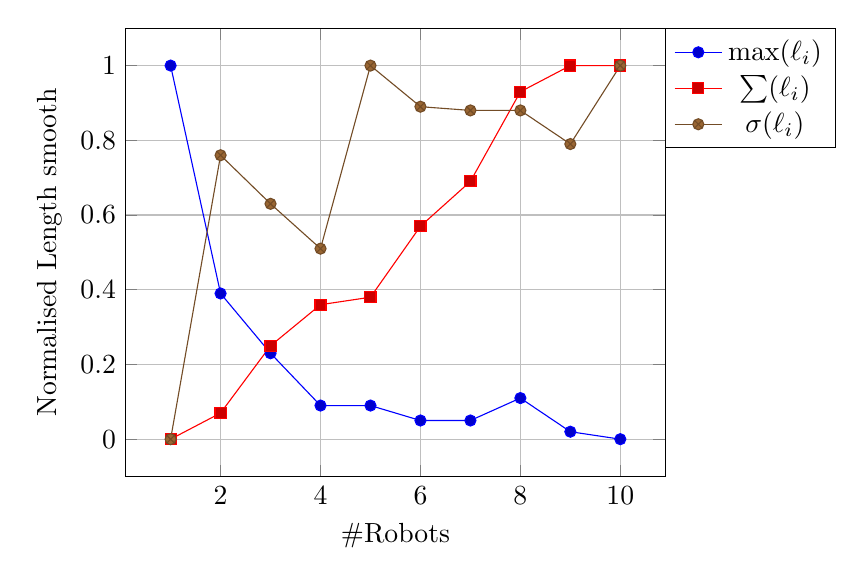
\begin{tikzpicture}
	\begin{axis}[
%		height=9cm,
%		width=9cm,
		grid=major,
                legend style = {at={(1,1)}, anchor=north west},
		xlabel=\#Robots,
		ylabel=Normalised Length
		smooth,
		tension=0.3
	]

	\addplot coordinates {
(1, 1.00)
(2, 0.39)
(3, 0.23)
(4, 0.09)
(5, 0.09)
(6, 0.05)
(7, 0.05)
(8, 0.11)
(9, 0.02)
(10, 0.00)
	};
	\addlegendentry{$\max(\ell_i)$}

	\addplot coordinates {
(1, 0.00)
(2, 0.07)
(3, 0.25)
(4, 0.36)
(5, 0.38)
(6, 0.57)
(7, 0.69)
(8, 0.93)
(9, 1.00)
(10, 1.00)
	};
	\addlegendentry{$\sum(\ell_i)$}

	\addplot coordinates {
(1, 0.00)
(2, 0.76)
(3, 0.63)
(4, 0.51)
(5, 1.00)
(6, 0.89)
(7, 0.88)
(8, 0.88)
(9, 0.79)
(10, 1.00)
	};
	\addlegendentry{$\sigma(\ell_i)$}
	\end{axis}
\end{tikzpicture}
\caption[Perform. indexes increasing the \#robots, city map using VRP]{\mbox{Performance indexes increasing the num. of robots, city map using VRP}}
\end{figure}

\begin{figure}[H]
\centering
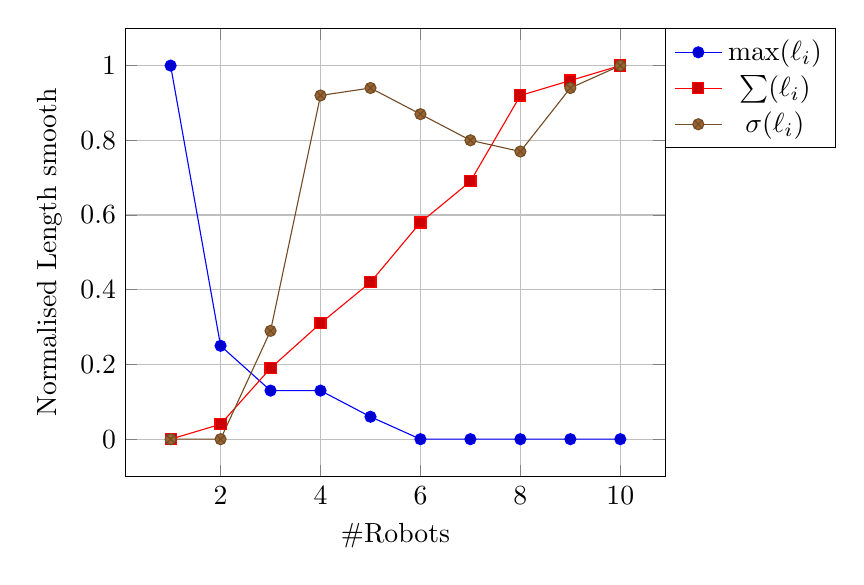
\begin{tikzpicture}
	\begin{axis}[
%		height=9cm,
%		width=9cm,
		grid=major,
                legend style = {at={(1,1)}, anchor=north west},
		xlabel=\#Robots,
		ylabel=Normalised Length
		smooth,
		tension=0.3
	]

	\addplot coordinates {
(1, 1.00)
(2, 0.25)
(3, 0.13)
(4, 0.13)
(5, 0.06)
(6, 0.00)
(7, 0.00)
(8, 0.00)
(9, 0.00)
(10, 0.00)
	};
	\addlegendentry{$\max(\ell_i)$}

	\addplot coordinates {
(1, 0.00)
(2, 0.04)
(3, 0.19)
(4, 0.31)
(5, 0.42)
(6, 0.58)
(7, 0.69)
(8, 0.92)
(9, 0.96)
(10, 1.00)
	};
	\addlegendentry{$\sum(\ell_i)$}

	\addplot coordinates {
(1, 0.00)
(2, 0.00)
(3, 0.29)
(4, 0.92)
(5, 0.94)
(6, 0.87)
(7, 0.80)
(8, 0.77)
(9, 0.94)
(10, 1.00)
	};
	\addlegendentry{$\sigma(\ell_i)$}
	\end{axis}
\end{tikzpicture}
\caption[Perform. indexes increasing the \#robots, 5x5 grid using VRP]{Performance indexes increasing the num. of robots, 5x5 grid using VRP}
\end{figure}

For the VRP algorithm we find that for a 5x5 map the best number of robots is 2, for the 10x10 map is 3 and for the 15x15 map is 5. We can clearly see how using this kind of algorithm the best number of robots is on average less than the one needed for Node Counting, that is a desirable property in term of resource saving.

\begin{figure}[H]
\centering
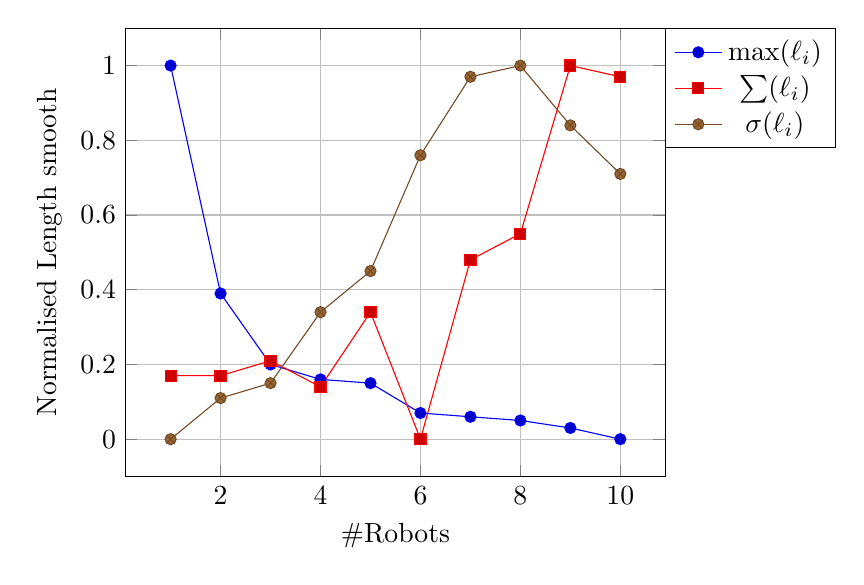
\begin{tikzpicture}
	\begin{axis}[
%		height=9cm,
%		width=9cm,
		grid=major,
                legend style = {at={(1,1)}, anchor=north west},
		xlabel=\#Robots,
		ylabel=Normalised Length
		smooth,
		tension=0.3
	]

	\addplot coordinates {
(1, 1.00)
(2, 0.39)
(3, 0.20)
(4, 0.16)
(5, 0.15)
(6, 0.07)
(7, 0.06)
(8, 0.05)
(9, 0.03)
(10, 0.00)
	};
	\addlegendentry{$\max(\ell_i)$}

	\addplot coordinates {
(1, 0.17)
(2, 0.17)
(3, 0.21)
(4, 0.14)
(5, 0.34)
(6, 0.00)
(7, 0.48)
(8, 0.55)
(9, 1.00)
(10, 0.97)
	};
	\addlegendentry{$\sum(\ell_i)$}

	\addplot coordinates {
(1, 0.00)
(2, 0.11)
(3, 0.15)
(4, 0.34)
(5, 0.45)
(6, 0.76)
(7, 0.97)
(8, 1.00)
(9, 0.84)
(10, 0.71)
	};
	\addlegendentry{$\sigma(\ell_i)$}
	\end{axis}
\end{tikzpicture}
\caption[Perform. indexes increasing the \#robots, 10x10 grid using VRP]{\mbox{Performance indexes increasing the num. of robots, 10x10 grid using NC}}
\end{figure}

\begin{figure}[H]
\centering
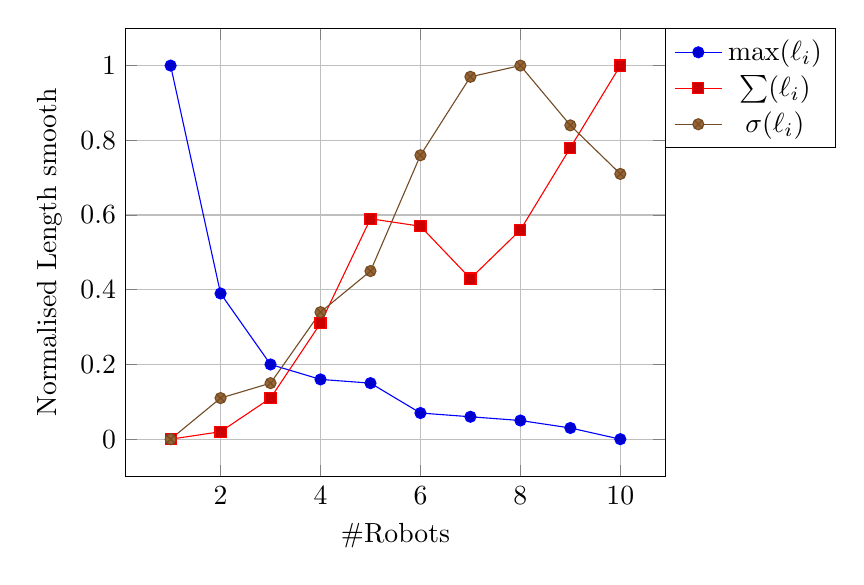
\begin{tikzpicture}
	\begin{axis}[
%		height=9cm,
%		width=9cm,
		grid=major,
                legend style = {at={(1,1)}, anchor=north west},
		xlabel=\#Robots,
		ylabel=Normalised Length
		smooth,
		tension=0.3
	]

	\addplot coordinates {
(1, 1.00)
(2, 0.39)
(3, 0.20)
(4, 0.16)
(5, 0.15)
(6, 0.07)
(7, 0.06)
(8, 0.05)
(9, 0.03)
(10, 0.00)
	};
	\addlegendentry{$\max(\ell_i)$}

	\addplot coordinates {
(1, 0.00)
(2, 0.02)
(3, 0.11)
(4, 0.31)
(5, 0.59)
(6, 0.57)
(7, 0.43)
(8, 0.56)
(9, 0.78)
(10, 1.00)
	};
	\addlegendentry{$\sum(\ell_i)$}

	\addplot coordinates {
(1, 0.00)
(2, 0.11)
(3, 0.15)
(4, 0.34)
(5, 0.45)
(6, 0.76)
(7, 0.97)
(8, 1.00)
(9, 0.84)
(10, 0.71)
	};
	\addlegendentry{$\sigma(\ell_i)$}
	\end{axis}
\end{tikzpicture}
\caption[Perform. indexes increasing the \#robots, 15x15 grid using VRP]{\mbox{Performance indexes increasing the num. of robots, 15x15 grid using NC}}
\end{figure}

In Fig. \ref{fig:VRPFW_execTime} is presented a comparison plot for the algorithm execution time with an increasing size of the maps.  The longest execution time has been recorded for the computation of the path for one robot in a 40 by 40 free map, for a value of $7\e{2}$ seconds, roughly 12 minutes \footnotemark[1].

\footnotetext[1]{On a 64-bit Intel\textsuperscript{\textregistered} Core\texttrademark ~i7-2670QM CPU @ 2.20GHz with a 6MB L3 Cache.}


\begin{figure}[H]
\centering
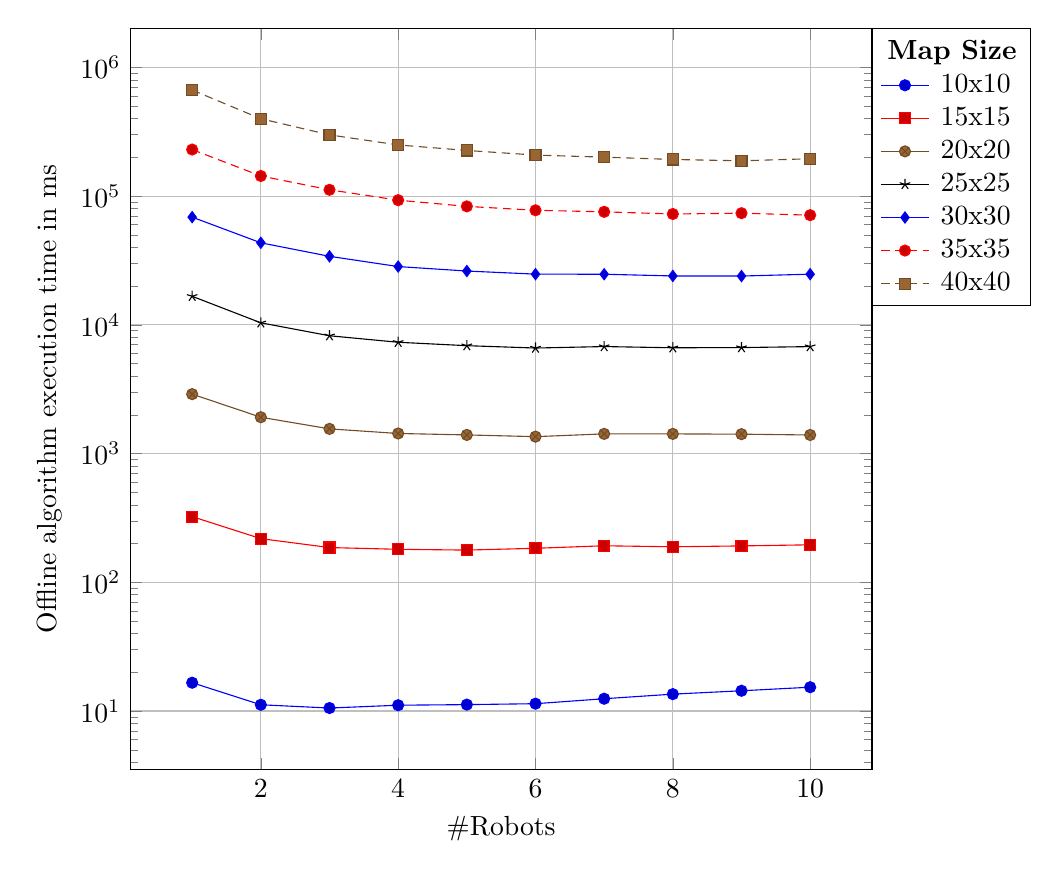
\begin{tikzpicture}
	\begin{semilogyaxis}[
		height=11cm,
		width=11cm,
                legend style = {at={(1,1)}, anchor=north west},
		grid=major,
		xlabel=\#Robots,
                   ylabel=Offline algorithm execution time in ms
	]

        \addlegendimage{empty legend}
        \addlegendentry{\hspace{-.6cm}\textbf{Map Size}}

%	\addplot coordinates {
%		(1, 0.962165)
%		(2, 0.999812)
%		(3, 3.32455)
%		(4, 1.33711)
%		(5, 1.26769)
%		(6, 4.00359)
%		(7, 4.45941)
%		(8, 1.33102)
%		(9, 1.38427)
%                (10, 3.06631)
%	};
%	\addlegendentry{5x5}

	\addplot coordinates {
		(1, 99.5812/6)
		(2, 67.1215/6)
		(3, 63.3223/6)
		(4, 66.5972/6)
		(5, 67.303/6)
		(6, 68.4257/6)
		(7, 74.7808/6)
		(8, 81.1845/6)
		(9, 86.226/6)
                (10, 91.9106/6)
	};
	\addlegendentry{10x10}

	\addplot coordinates {
		(1, 1941.57/6)
		(2, 1310.12/6)
		(3, 1117.07/6)
		(4, 1082.52/6)
		(5, 1067.53/6)
		(6, 1102.4/6)
		(7, 1153.16/6)
		(8, 1132.38/6)
		(9, 1150.22/6)
                (10, 1173.2/6)
	};
	\addlegendentry{15x15}

	\addplot coordinates {
		(1, 17361.1/6)
		(2, 11490/6)
		(3, 9328.54/6)
		(4, 8591.75/6)
		(5, 8372.56/6)
		(6, 8116.5/6)
		(7, 8529.95/6)
		(8, 8526.77/6)
		(9, 8485.28/6)
                (10, 8361.64/6)
	};
	\addlegendentry{20x20}

	\addplot coordinates {
		(1, 99929.9/6)
		(2, 62180.2/6)
		(3, 49326.2/6)
		(4, 43910.5/6)
		(5, 41311.1/6)
		(6, 39607.3/6)
		(7, 40667/6)
		(8, 39792/6)
		(9, 39942.7/6)
                (10,40629.5/6)
	};
	\addlegendentry{25x25}

	\addplot coordinates {
		(1, 411589/6)
		(2, 260044/6)
		(3, 204265/6)
		(4, 170023/6)
		(5, 156969/6)
		(6, 148516/6)
		(7, 148225/6)
		(8, 143764/6)
		(9, 143510/6)
                (10, 148387/6)
	};
	\addlegendentry{30x30}

	\addplot coordinates {
		(1, 1.37889e+06/6)
		(2, 859312/6)
		(3, 671124/6)
		(4, 557420/6)
		(5, 498969/6)
		(6, 465257/6)
		(7, 452598/6)
		(8, 435339/6)
		(9, 441815/6)
                (10, 426400/6)
	};
	\addlegendentry{35x35}

	\addplot coordinates {
		(1, 3.99748e+06/6)
		(2, 2.39203e+06/6)
		(3, 1.79249e+06/6)
		(4, 1.49702e+06/6)
		(5, 1.35637e+06/6)
		(6, 1.24861e+06/6)
		(7, 1.20327e+06/6)
		(8, 1.15456e+06/6)
		(9, 1.12716e+06/6)
                (10, 1.16961e+06/6)
	};
	\addlegendentry{40x40}
	
	\end{semilogyaxis}
\end{tikzpicture}
\caption{VRP-FloydWarshall:  Different execution times for growing map sizes}
\label{fig:VRPFW_execTime}
\end{figure}








\pagebreak


\section{Conclusions}
We have seen how for the multi-robot coverage problem the elementary Node Counting algorithm resulted to be one of the most efficient solutions, with final paths lengths even comparable with the VRP Greedy ones. The most interesting results being the one of the ``vertex oriented'' algorithms Node Counting and LRTA*, the latter suffering for the intrinsic inefficient mechanism implemented for the update rule in the multi-robot case (section \ref{sec:LRTAstar}). ``Edge oriented'' algorithm as Edge Counting and PatrolGRAPH* do not seem to fit the needs of the coverage problem as they always end up in longer paths with respected to the vertex oriented algorithms.
The VRP algorithm seems anyway to achieve the overall best results in very large obstacle-free maps, which can be the case for high altitude flight. An undeniable advantage of the VRP algorithm also is that the solution is almost instant giving us an idea of the total coverage time, a very useful information in SAR applications.


